\documentclass{beamer}
\hypersetup{breaklinks=false}
\usepackage{amsmath,amsfonts,amssymb}
\setbeamertemplate{footline}[frame number]
\usetheme{Warsaw}  %% Themenwahl
\usepackage{color}

\title[Multi-purpose Library of Recommender System Algorithms]
{Multi-purpose Library of Recommender System Algorithms for the Item Prediction Task}
\subtitle{Presentation of my Bachelor Thesis}
\author{Julius Kolbe}
\institute{Fakult\"at f\"ur Elektrotechnik und Informatik\\Institut f\"ur Verteilte Systeme}
\date{\today}
\usepackage{pdfpages}
\usepackage{listings}
\lstdefinestyle{pseudocode}{%language=Python,
    keywordstyle=\color{RoyalBlue},%\bfseries,
    basicstyle=\small\ttfamily,
    %identifierstyle=\color{NavyBlue},
    commentstyle=\color{Green}\ttfamily,
    stringstyle=\rmfamily,
    numbers=none,%left,%
    numberstyle=\scriptsize,%\tiny
    stepnumber=5,
    numbersep=8pt,
    showstringspaces=false,
    breaklines=true,
    frameround=ftff,
    frame=single,
    belowcaptionskip=.75\baselineskip
    %frame=L
} 



\usepackage{tikz}
\usetikzlibrary{fit,shapes.misc}

\newcommand\marktopleft[1]{%
    \tikz[overlay,remember picture] 
    \node (marker-#1-a) at (0,1.5ex) {};%
}
\newcommand\markbottomright[2][red]{%
    \tikz[overlay,remember picture] 
    \node (marker-#2-b) at (0,0) {};%
    \tikz[overlay,remember picture,thick,inner sep=3pt,fill=red]
    \node[draw,rectangle,fill=#1,nearly transparent,fit=(marker-#2-a.center) (marker-#2-b.center)] {};%
}

\begin{document}
\frame{\titlepage} % overview over the thesis with reference to recsyslab as major contribution.
%\frame{\tableofcontents[currentsection]}
\frame{
    \frametitle{Contents}
    \tableofcontents
   % [pausesections]
}

\section{Background}
\frame{
    \frametitle{Contents}
    \tableofcontents[currentsection]
   % [pausesections]
}
\subsection{Item Prediction Task and Implicit Feedback}
\begin{frame}
\frametitle{Implicit Feedback}

\begin{table}[t]
\begin{tabular}{c|cccccc}
    &Anna&Berta&Claudia&Dagmar\\\hline
    The Shawshank Redemption&1&&1&\\
    The Godfather&&1&1&\\
    The Godfather: Part II&&1&&1\\
    Pulp Fiction&1&1&&1\\
    The Good, the Bad and the Ugly&1&&1&\\
\end{tabular}
\end{table}
% Consider the following scenario where we have a viewing history of some persons as illustrated here. [vorlesen]
% We also call this implicit feedback because the women weren't ask to rate the movies
% they just watched them and we're trying to get some useful information out of it.
% The item prediction task a recommender has to solve is to predict which movies are interesting for which persons
\end{frame}
\begin{frame}
\frametitle{Item Prediction Task}

\begin{table}[t]
\begin{tabular}{c|cccccc}
    &Anna&Berta&Claudia&Dagmar\\\hline
    The Shawshank Redemption&1&&1&?\\
    The Godfather&&1&1&?\\
    The Godfather: Part II&&1&&1\\
    Pulp Fiction&1&1&&1\\
    The Good, the Bad and the Ugly&1&&1&?\\
\end{tabular}
% So for example when dagmar goes to the cinema, which movie should we recommend her?
% Here it's quite probably The Godfather to she should see, but normally those systems
% are used in scenarios with thousands of persons and movies.
\end{table}

\end{frame}
\begin{frame}

\frametitle{Notation}

\begin{table}[t]
    \begin{tabular}{c|cccccc}
        &\marktopleft{c2}Anna&Berta&Claudia&Dagmar\markbottomright[red]{c2}\\\hline
        \marktopleft{c3}The Shawshank Redemption&\marktopleft{c1}1&&1&\\
        The Godfather&&\marktopleft{c4}1&1&\\
        The Godfather: Part II&&1&&1\\
        Pulp Fiction&1&1\markbottomright[magenta]{c4}&&1\\
        The Good, the Bad and the Ugly\markbottomright[green]{c3}&1&&1&\markbottomright[blue]{c1}\\
\end{tabular}
\end{table}
%From now on I will refer to those with:
\textcolor{green}{Items}\\
\textcolor{red}{Users}\\
\textcolor{blue}{Interactions}\\
\textcolor{magenta}{Basket of $u$}
% Please note, that it is not important what exactly they are.
% Interactions can be purchases, views, clicks etc
% and then the items will be for example goods to buy or videos.

\end{frame}
\subsection{Evaluation}
\begin{frame}
    \frametitle{Leave-one-out Protocol}
    \begin{enumerate}
        \item Randomly choose one interaction per user and hide them
        \item Train the recommender system with the remaining interactions
        \item Get recommendations for every user
        \item Compute the chosen evaluation metric with the hidden items and the recommendations
    \end{enumerate}

\end{frame}
\subsection{Evaluation Metrics}
\begin{frame} 
\frametitle{Hitrate/Recall@N~\cite{Karypis:2001:EIT:502585.502627, Sarwar00applicationof}}
\begin{equation} 
\text{Recall@N}=\frac{\sum_{u \in U} H_u \cap \text{topN}_u}{|H|}
\end{equation}\\
\vspace{6.4mm}
\begin{description}
    \item[$H$] hidden interactions\\
    \item[$H_u$] the hidden interaction of $u$\\
    \item[$U$] set of users
    \item[$topN_u$] N recommendations for $u$
\end{description}
\end{frame}

\begin{frame} 
\frametitle{Precision~\cite{Sarwar00applicationof}}
\begin{equation} 
\text{Precision}=\frac{\sum_{u \in U} H_u \cap \text{topN}_u}{N \times |U|}
\end{equation}\\
\vspace{6.4mm}
\begin{description}
    \item[$H$] hidden interactions\\
    \item[$H_u$] the hidden interaction of $u$\\
    \item[$U$] set of users
    \item[$topN_u$] $N$ recommendations for $u$
\end{description}
\end{frame}

\begin{frame} 
    \frametitle{F1~\cite{Sarwar00applicationof}}
\begin{equation} 
\text{F1}=\frac{2 \times \text{Recall@N} \times 
\text{Precision}}{\text{Recall@N} + \text{Precision}}.
\end{equation}\\
\vspace{6.4mm}
\begin{description}
    \item[$H$] hidden interactions\\
    \item[$H_u$] the hidden interaction of $u$\\
    \item[$U$] set of users
    \item[$topN_u$] $N$ recommendations for $u$
\end{description}
\end{frame}

\begin{frame} 
    \frametitle{Mean Reciprocal Hitrate~\cite{DBLP:conf/icdm/NingK11}}
\begin{equation} 
\text{MRHR}=\frac{1}{|U|} \sum_{u \in U} \frac{1}{\text{pos}(\text{topN}_{u},H_{u})},
\end{equation}\\
\vspace{6.4mm}
\begin{description}
    \item[$H$] hidden interactions\\
    \item[$H_u$] the hidden interaction of $u$\\
    \item[$U$] set of users
    \item[$topN_u$] $N$ recommendations for $u$
    \item[$\text{pos}(\text{topN}_{u},H_{u})$] position of the hidden item in the list of recommendations
\end{description}
\end{frame}

\begin{frame} 
    \frametitle{Area under the ROC (AUC)~\cite{Rendle:2009:BBP:1795114.1795167}}
\begin{equation} 
\text{AUC}=\frac{1}{|U|}\sum_{u \in U} \frac{1}{|E(u)|} 
\sum_{(i,j) \in E(u)} \delta(x_{ui}>x_{uj}),
\end{equation}\\
\begin{equation}
\delta(x)=\begin{cases}1, & \text{if x is true}, \\
                       0, & \text{otherwise.}
\end{cases}
\end{equation}
\begin{equation}
E(u) =\{(i,j)|(u,i) \in H \land (u,j) \not\in (H \cup T)\}.
\end{equation}
%\vspace{6.4mm}
\begin{description}
    \item[$H$] hidden interactions\\
    \item[$H_u$] the hidden interaction of $u$\\
    \item[$U$] set of users
    \item[$x_{ui}$] predicted score of the interaction between $u$ and $i$
\end{description}
\end{frame}

\section{Recommendation Algorithms}
\frame{
    \frametitle{Contents}
    \tableofcontents[currentsection]
}
\begin{frame}
\frametitle{Non-Personalized}
\begin{description}
    \item[Constant] Recommend the most popular items
    \item[Random] Recommend randomly chosen items
\end{description}
\end{frame}
\begin{frame}
\frametitle{k-Nearest-Neighbor~\cite{Karypis:2001:EIT:502585.502627}}
\begin{enumerate}
    \item Compute similarity of each item, item pair
    \item For each item, save the $k$ items with the highest similarity\\(= neighbors)
    \item Compute the union of the neighbors of the basket of $u$
    \item For each item in this set compute the sum of similarities to the basket of $u$
    \item Sort by this score and return the first $N$ items
\end{enumerate}
\begin{equation}
    \text{sim}(i,j) = \cos(\vec{i}, \vec{j})=\frac{\vec{i} \cdot \vec{j}}{||\vec{i}||_{2} ||\vec{j}||_{2}}
\end{equation}
% This is item based but it can also be done user based.
\end{frame}
\begin{frame}
\frametitle{k-Nearest-Neighbor~\cite{Karypis:2001:EIT:502585.502627}}
\begin{table}[t]
\begin{tabular}{c|cccccc}
    &Anna&Berta&Claudia&Dagmar\\\hline
    The Shawshank Redemption&\marktopleft{c5}1&0&1&0\markbottomright[red]{c5}\\
    The Godfather&0&1&1&0\\
    The Godfather: Part II&\marktopleft{c7}0&1&0&1\markbottomright[green]{c7}\\ 
    Pulp Fiction&1&1&0&1\\
    The Good, the Bad and the Ugly&1&0&1&0\\
\end{tabular}
\end{table}
\begin{equation*}
    \text{sim}(i,j) = \cos(\vec{i}, \vec{j})=\frac{\vec{i} \cdot \vec{j}}{||\vec{i}||_{2} ||\vec{j}||_{2}}
    = \frac{0}{2}=0
\end{equation*}
\end{frame}
\begin{frame}
\frametitle{k-Nearest-Neighbor~\cite{Karypis:2001:EIT:502585.502627}}
\begin{table}[t]
\begin{tabular}{c|cccccc}
    &Anna&Berta&Claudia&Dagmar\\\hline
    The Shawshank Redemption&1&0&1&0\\
    The Godfather&0&1&1&0\\
    The Godfather: Part II&\marktopleft{c7}0&1&0&1\markbottomright[green]{c7}\\
    Pulp Fiction&\marktopleft{c8}1&1&0&1\markbottomright[blue]{c8}\\
    The Good, the Bad and the Ugly&1&0&1&0\\
\end{tabular}
\end{table}
\begin{equation*}
    \text{sim}(i,j) = \cos(\vec{i}, \vec{j})=\frac{\vec{i} \cdot \vec{j}}{||\vec{i}||_{2} ||\vec{j}||_{2}}
    =\frac{2}{\sqrt{2}\sqrt{3}}
\end{equation*}
% go back again and explain the rest of the algorithm.
\end{frame}
\begin{frame}
    \frametitle{Matrix Factorization~\cite{matrixfactorization}}
\begin{table}[t]
\begin{tabular}{c|cccccc}
    &Anna&Berta&Claudia&Dagmar\\\hline
    The Shawshank Redemption&\marktopleft{c9}1&0&1&0\\
    The Godfather&0&1&1&0\\
    The Godfather: Part II&0&1&0&1\\
    Pulp Fiction&1&1&0&1\\
    The Good, the Bad and the Ugly&1&0&1&0\markbottomright[green]{c9}\\
\end{tabular}
\end{table}
\begin{center}
Find $W$ and $H$ so:
\(\textcolor{green}{\hat{M}} = W\;H^\top\).\\
        \begin{equation}
    \text{Score}(u,i) = W_u I_i^\top.
\end{equation}
\end{center}
%explain the transpose
%explain that W and H are features of the items and the features
\end{frame}
\begin{frame}[fragile]
    \frametitle{Matrix Factorization, Training}
\begin{lstlisting}[style=pseudocode]
U = randomly chosen user
I = randomly chosen item U interacted with
J = randomly chosen item U did not interact with

X=H[i] - H[j]
wx = dot product of W[u] and X
dloss = (derivative of the 
        loss function of wx and 1) * 
        learningRate
        
W[u] += dloss * (H[i] - H[j]) #These three lines
H[i] += dloss * W[u]          #have to be
H[j] += dloss * -W[u]         #executed at once
\end{lstlisting}
\end{frame}
%\begin{frame}
%\frametitle{Slope One~\cite{DBLP:journals/corr/abs-cs-0702144}}
%\begin{table}[t]
%\begin{tabular}{c|cccccc}
%    &Anna&Berta&Claudia&Dagmar\\\hline
%    The Shawshank Redemption&1&&1&\\
%    The Godfather&&1&1&\\
%    The Godfather: Part II&&1&&1\\
%    Pulp Fiction&\marktopleft{c10}1&1&2&1\markbottomright[green]{c10}\\
%    The Good, the Bad and the Ugly&\marktopleft{c11}2&?&1&3\markbottomright[red]{c11}\\
%\end{tabular}%database changed so slope one works.
%\end{table}
%\begin{equation}
%
%\end{equation}
%\end{frame}
%should i include slopeone? it doesn't work great and is complicated to explain.

\section{Recsyslab}
\frame{
    \frametitle{Contents}
    \tableofcontents[currentsection]
   % [pausesections]
}
\begin{frame} 
\frametitle{Introduction of recsyslab} %also comparison with other frameworks
\begin{itemize}
    \item Python for easy readable source code
    \item simple usage
    \item for education
    \item for research
    \item open source license: GPLv3
\end{itemize}
\end{frame}
\begin{frame}
\frametitle{General Structure}
\begin{center}
    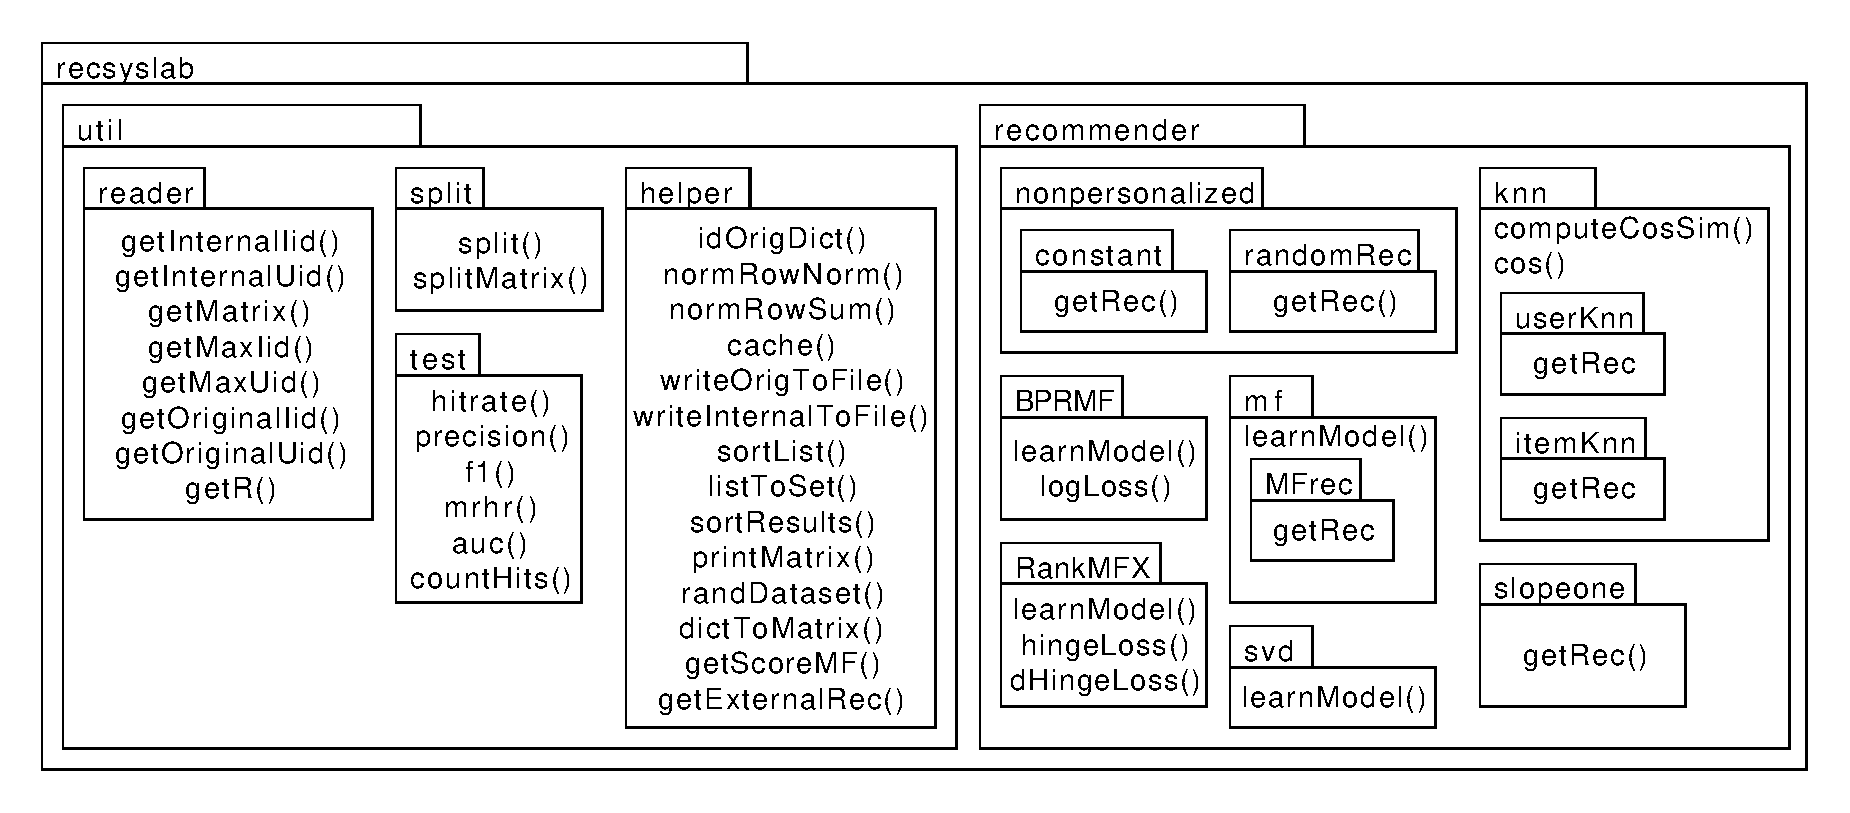
\includegraphics[page=1, scale=0.3]{packagediagram.pdf}
%    \hspace*{8cm}
\end{center}
\end{frame}
\begin{frame}[fragile]
    \frametitle{Get recsyslab}
%    Github repository:\\
    \url{github.com/Foolius/recsyslab}\\
    \hspace*{8cm}\\
%    Direct download of a .zip:\\
    \url{github.com/Foolius/recsyslab/archive/master.zip}\\
    \hspace*{8cm}\\
%    Clone it with git:
    \begin{lstlisting}[style=pseudocode]
$ git clone 
    https://github.com/Foolius/recsyslab.git
    \end{lstlisting}
\end{frame}

\bibliographystyle{plainnat}
\bibliography{Bibliography}
\end{document}
